\documentclass[crop,tikz]{standalone}

\usepackage{tikz}
\usepackage{anyfontsize}

\usetikzlibrary{bending}
\usetikzlibrary{arrows.meta}
\begin{document}

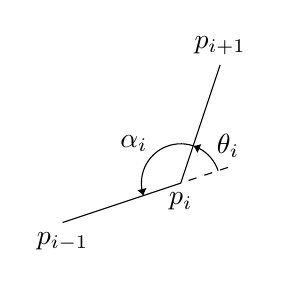
\begin{tikzpicture}

\node [below] at (0,0) {$p_{i-1}$};
\draw (0,0) -- (1.5,0.5);
\node [below] at (1.5,0.5) {$p_i$};
\draw (1.5,0.5) -- (2,2);
\node [above] at (2, 2) {$p_{i+1}$};

\draw[dashed, shorten <=3] (1.5,0.5) -- (2.1, 0.7);
\draw [arrows = {-Latex[scale length=0.5]}] ([shift=(18.5:0.5)]1.5,0.5) arc [radius=0.5, start angle=18.5, end angle= 71.5];
\node [above] at (2.1, 0.7) {$\theta_i$};
\draw [arrows = {-Latex[scale length=0.5]}] ([shift=(71.5:0.5)]1.5,0.5) arc [radius=0.5, start angle=71.5, end angle= 198.5];
\node [left] at (1.2, 1) {$\alpha_i$};

\end{tikzpicture}

\end{document}